\section{Linha do tempo}
\label{sec:cap4_linha_tempo}

Antes da exibição do resultados, será apresentada a linha do tempo da missão de \gls{rvdb}.
Nela será possível observar quando e o que acontece em cada momento importante da simulação da missão deste trabalho.
Para melhor eficiência computacional, a simulação realizada na plataforma Matlab/Simulink foi separada conforme as aproximações realizadas, portanto, inicialmente simulou-se a aproximação de longa distância por completo, posteriormente a aproximação de curta distância e em paralelo, a aproximação final.

\begin{figure}[H]
\centering
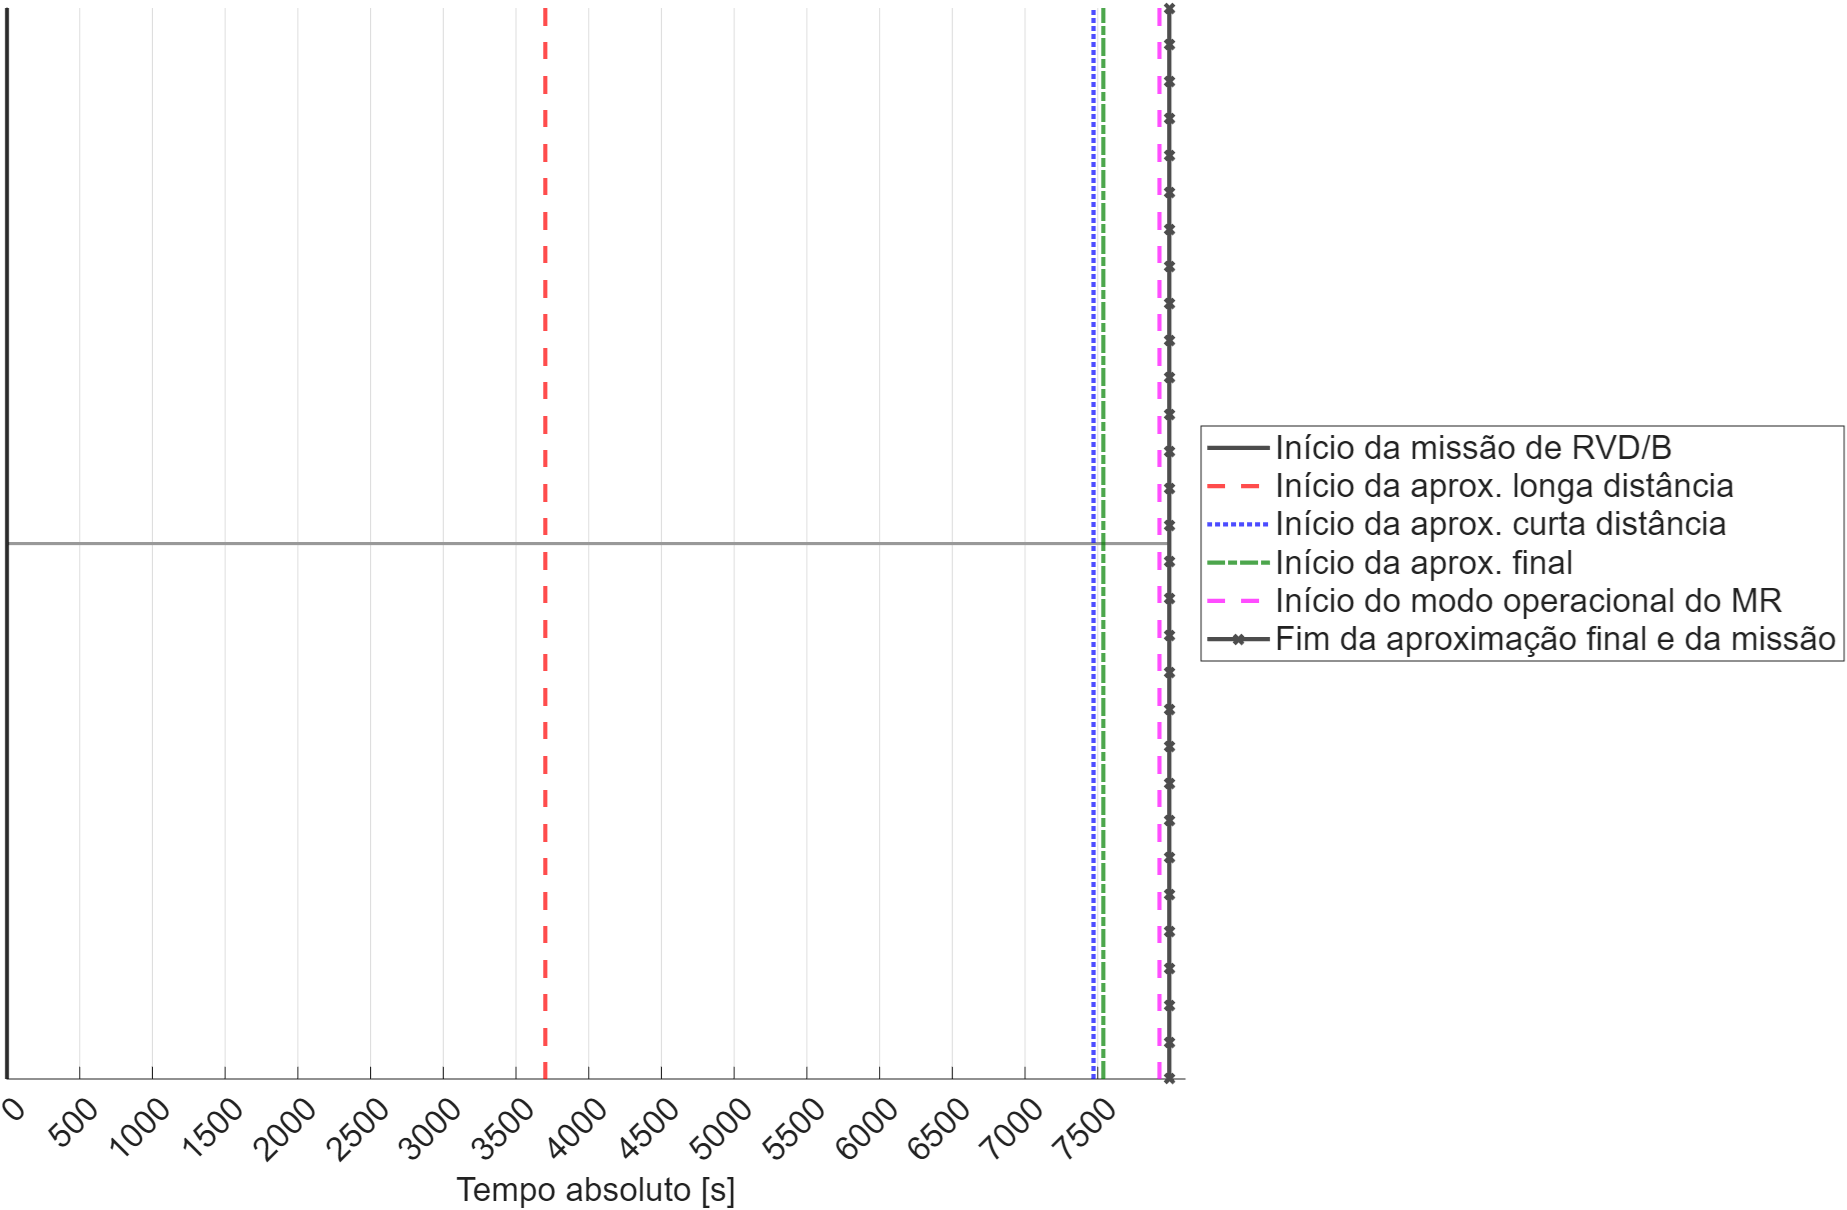
\includegraphics[width=1\linewidth]{4 Resultados e discussoes/Imagens/Linha do tempo.png}
\caption{Linha do tempo da missão de \gls{rvdb}}
    \label{fig:cap4_linha_tempo}
\end{figure}

A Figura~\ref{fig:cap4_linha_tempo} e a Tabela~\ref{tab:cap4_linha_tempo} sintetizam os principais marcos temporais da missão, indicando para cada evento o instante correspondente em segundos e em horas.
Entre o início da missão de \gls{rvdb} ($t = 0$ s) e o início da aproximação de longa distância ($t = 3.702$ s) ocorre a redução da diferença de fase entre perseguidor e alvo, preparando a condição adequada para a transferência orbital.

Em seguida, após o final da aproximação de longa distância no instante $t = 6.571$ s, tem início o trecho de \emph{drift} orbital, que se estende até $t = 7.471$ s, quando se inicia a aproximação de curta distância. Esta, por sua vez, evolui até o instante $t = 7.538$ s, momento em que se caracteriza o início da aproximação final e em que a dinâmica do corpo rígido ainda é descrita pela formulação de Euler.

No instante $t = 7.924$ s é realizada a comutação entre as dinâmicas, passando-se a empregar o modelo acoplado de base flutuante descrito pelas equações de Lagrange, e o \gls{mr} entra em operação para conduzir a ferramenta até a porta de acoplamento. Por fim, em $t = 7.992$ s considera-se encerrada a missão, uma vez que a ferramenta se encontra engatada e estabilizada, dispensando correções adicionais de atitude ou de posição fina.

\begin{table}[H]
\centering
\caption{Linha do tempo da missão e das fases de aproximação.}
\label{tab:cap4_linha_tempo}
\begin{tabularx}{\linewidth}{|
  >{\raggedright\arraybackslash}X|
  >{\centering\arraybackslash}X|
  >{\centering\arraybackslash}X|}
\hline
\textbf{Evento} &
\textbf{Tempo [s]} &
\textbf{Tempo [h]} \\
\hhline{|=|=|=|}
Início da missão &
$0$ & $00\text{h }00\text{min }00\text{s}$ \\
\hline
Início da aproximação longa distância ($\Delta v1$) & $3.702$ & $01\text{h }01\text{min }41\text{s}$ \\
\hline
Final da aproximação longa distância ($\Delta v2$) & $6.571$ & $01\text{h }49\text{min }30\text{s}$ \\
\hline
Início da aproximação curta distância &$7.471$ & $02\text{h }04\text{min }30\text{s}$ \\
\hline
Início da aproximação final & $7.538$ & $02\text{h }05\text{min }38\text{s}$ \\
\hline
Comutação entre as dinâmicas & $7.924$ & $02\text{h }12\text{min }04\text{s}$ \\
\hline
Fim da aproximação final & $7.992$ & $02\text{h }13\text{min }11\text{s}$ \\
\hline
\textbf{Tempo total da missão} & $7.992$ & $02\text{h }13\text{min }11\text{s}$ \\
\hline
\end{tabularx}
\end{table}

\subsection{Comparativo entre cenários}

De forma análoga ao cenário de referência, o Cenário (B) mantém a mesma sequência de fases da missão de \gls{rvdb}, porém deslocada para um tempo absoluto mais avançado.
Observa-se que o início da aproximação longa distância ocorre em $t = 31.134$ s, isto é, significativamente após o primeiro caso, bem como o início da aproximação curta ($t = 34.872$ s) e o início da aproximação final ($t = 34.940$ s). A duração do \emph{drift} orbital permanece igual a $900$ s, e a duração total da aproximação curta e da aproximação final é mantida, resultando em um tempo total de missão de $35.393$ s no Cenário B, em contraste com os $7.992$ s do cenário inicial. Em termos de estrutura temporal relativa, os intervalos entre eventos principais são preservados, mudando apenas o instante absoluto em que cada fase é executada.

\begin{table}[H]
\centering
\caption{Linha do tempo da missão e das fases de aproximação -- Cenário B.}
\label{tab:cap4_linha_tempo_B}
\begin{tabularx}{\linewidth}{|
  >{\raggedright\arraybackslash}X|
  >{\centering\arraybackslash}X|
  >{\centering\arraybackslash}X|}
\hline
\textbf{Evento} &
\textbf{Tempo [s]} &
\textbf{Tempo [h]} \\
\hhline{|=|=|=|}
Início da missão  & $0$ & $00\text{h }00\text{min }00\text{s}$ \\
\hline
Início da aproximação longa distância ($\Delta v1B$) &$31.134$ &$08\text{h }38\text{min }54\text{s}$ \\
\hline
Final da aproximação longa distância ($\Delta v2B$) &$33.972$ &$09\text{h }26\text{min }12\text{s}$ \\
\hline
% Duração do drift orbital  &$900$ &$00\text{h }15\text{min }00\text{s}$ \\
% \hline
% Final do drift orbital  &$34.872$ &$09\text{h }41\text{min }12\text{s}$ \\
% \hline
Início da aproximação curta distância  &$34.872$ &$09\text{h }41\text{min }12\text{s}$ \\
\hline
% Fim da aproximação curta distância  &$34.940$ &$09\text{h }42\text{min }19\text{s}$ \\
% \hline
Início da aproximação final  &$34.940$ &$09\text{h }42\text{min }19\text{s}$ \\
\hline
Comutação entre as dinâmicas & $35.325$ & $09\text{h }48\text{min }45\text{s}$ \\
\hline
Fim da aproximação final  &$35.393$ &$09\text{h }49\text{min }52\text{s}$ \\
\hline
\textbf{Tempo total da missão}  &$35.393$ &$09\text{h }49\text{min }52\text{s}$ \\
\hline
\end{tabularx}
\end{table}
